\documentclass[12pt]{article}

\usepackage{amsmath}
\usepackage{amssymb}
\usepackage[dvips]{graphicx}
%\usepackage{lscape}
\usepackage{eepic}
\usepackage{color}
\usepackage{wasysym} % \female \male
\usepackage[landscape,pdftex]{geometry}
\usepackage{fancyhdr}

\DeclareOption{bigsym}{\DeclareSymbolFont{largesymbols}{OMX}{psycm}{m}{n}}
\ProcessOptions

\setlength{\oddsidemargin}{-0.75in}
\setlength{\evensidemargin}{-0.75in}
\setlength{\topmargin}{-1in}
\setlength{\textheight}{7.75in}
\setlength{\textwidth}{10.5in}
\setlength{\footskip}{0in}
\setlength{\parindent}{0pt}
\setlength{\rightskip}{0pt plus 1fil} % makes ragged right

\renewcommand{\familydefault}{phv} % helvetica

% following: color
%\definecolor{mybgcolor}{rgb}{0,0,0.3125}
%\definecolor{myyellow}{rgb}{1,1,0.4}
%\definecolor{myblue}{rgb}{0.4,0.8,1}
%\definecolor{mypink}{rgb}{1,0.4,1}
%\definecolor{myhotpink}{rgb}{1,0,0.5}
%\definecolor{mywhite}{rgb}{1,1,1}

% following: B/W
\definecolor{mybgcolor}{rgb}{1,1,1}
\definecolor{myyellow}{rgb}{0,0,0}
\definecolor{myblue}{rgb}{0,0,0}
\definecolor{mypink}{rgb}{0,0,0}
\definecolor{myhotpink}{rgb}{0,0,0}
\definecolor{mywhite}{rgb}{0,0,0}

% header/footer layout
\pagestyle{fancy}
\lhead{} \chead{} \rhead{}
\lfoot{} \cfoot{} \rfoot{\color{myyellow} \thepage}
\renewcommand{\headrulewidth}{0pt}
\renewcommand{\footrulewidth}{0pt}

% font sizes
\newcommand{\superlarge}{\fontsize{60}{60} \selectfont}
\newcommand{\titlesize}{\fontsize{40}{50} \selectfont}
\newcommand{\headsize}{\fontsize{35}{35} \selectfont}
\newcommand{\textsize}{\fontsize{30}{35} \selectfont}
\newcommand{\smallsize}{\fontsize{25}{30} \selectfont}
\newcommand{\smallersize}{\fontsize{20}{25} \selectfont}
\newcommand{\smallestsize}{\fontsize{18}{22} \selectfont}
\newcommand{\lod}{\text{LOD}}
\newcommand{\plod}{\text{pLOD}}
\newcommand{\bic}{\text{BIC}}
\newcommand{\rss}{\text{RSS}}
\newcommand{\var}{\text{var}}
\newcommand{\M}{\text{M}}
%\renewcommand{\log}{\text{log}}
%\renewcommand{\max}{\text{max}}



\pagecolor{mybgcolor}
\color{mywhite}

\begin{document}

\thispagestyle{empty}

\begin{center}
\titlesize \color{myyellow}

\vspace*{15mm}

Haley-Knott regression

\color{mypink}
\rule{10in}{1mm}
%\vspace{-10mm}

\vspace{5mm}

\textsize \color{myblue}
Karl W Broman
\vspace{5mm}

\color{mywhite}
{\smallsize Department of Biostatistics and Medical Informatics

University of Wisconsin -- Madison
\vspace{20mm}


\verb|www.biostat.wisc.edu/~kbroman| \\
{\smallestsize \color{myblue} 
[$\rightarrow$ Teaching $\rightarrow$ Miscellaneous lectures]}
}

\end{center}

%\vfill
%
\includegraphics[height=1in]{Figs/qrcode_jax.png}

\newpage

\addtocounter{page}{+1}

\headsize \color{myyellow}
\hfill \begin{minipage}{5.75in}
\centering
Haley-Knott regression
\end{minipage}

\vspace{3cm}

\color{mywhite} \smallsize

\hspace*{0.5in}
A quick approximation to Interval Mapping.

\smallersize

\begin{eqnarray*}
\mathsf{E(y_i | q_i)} & = & \mathsf{ \mu_q } \\[24pt]
\mathsf{E(y_i | M_i)} & = & \mathsf{E[ \ E(y_i|q_i) \ | M_i]} 
 =  \mathsf{\textstyle{\sum_j \Pr(q=j|M_i) \mu_j}} \\[12pt]
& = & \mathsf{\textstyle{\sum_j p_{ij} \mu_j}}
\end{eqnarray*}

\vspace{1cm}

\hfill \begin{minipage}{10in}
\setlength{\rightskip}{0pt plus 1fil} % makes ragged right
{\color{mypink} Regress $\mathsf{y}$ on $\mathsf{p_i}$}, pretending the residual
variation is normally distributed (with constant variance).
\end{minipage}

\begin{eqnarray*}
\mathsf{\lod} & = & \mathsf{\frac{n}{2} \log_{10} \left( \frac{\rss_0}{\rss_1} \right)}
\end{eqnarray*}

\newpage

\headsize \color{myyellow}
\hfill \begin{minipage}{5.75in}
\centering
The normal mixtures
\end{minipage}

\vspace{15mm}

\hspace*{0.5in}
\begin{minipage}[t]{4.6in}
\vspace*{10mm}

\color{mywhite} \smallersize 
\setlength{\unitlength}{1.0in}
\begin{center}
\begin{picture}(4.5,1)
% lines
\Thicklines
\put(0.25,0.5){\line(1,0){4}}
\put(0.25,0.35){\line(0,1){0.3}}
\put(1.65,0.35){\line(0,1){0.3}}
\put(4.25,0.35){\line(0,1){0.3}}

% text
\put(0.25,0.1){\makebox(0,0){$\mathsf{M_1}$}}
\put(4.25,0.1){\makebox(0,0){$\mathsf{M_2}$}}
\put(1.65,0.1){\makebox(0,0){$\mathsf{Q}$}}
\put(0.95,0.8){\makebox(0,0){7 cM}}
\put(2.95,0.8){\makebox(0,0){13 cM}}
\end{picture} \end{center}
\vspace{5mm}

\begin{itemize}
\setlength{\rightskip}{0pt plus 1fil} % makes ragged right
\item Two markers separated by 20 cM, with the QTL closer to the left marker.
\item The figure at right shows the distributions of the phenotype
conditional on the genotypes at the two markers.
\item The dashed curves correspond to the components of the mixtures.
\end{itemize}

\end{minipage}
\hfill
\begin{minipage}[t]{4.6in}
\vspace*{0mm}

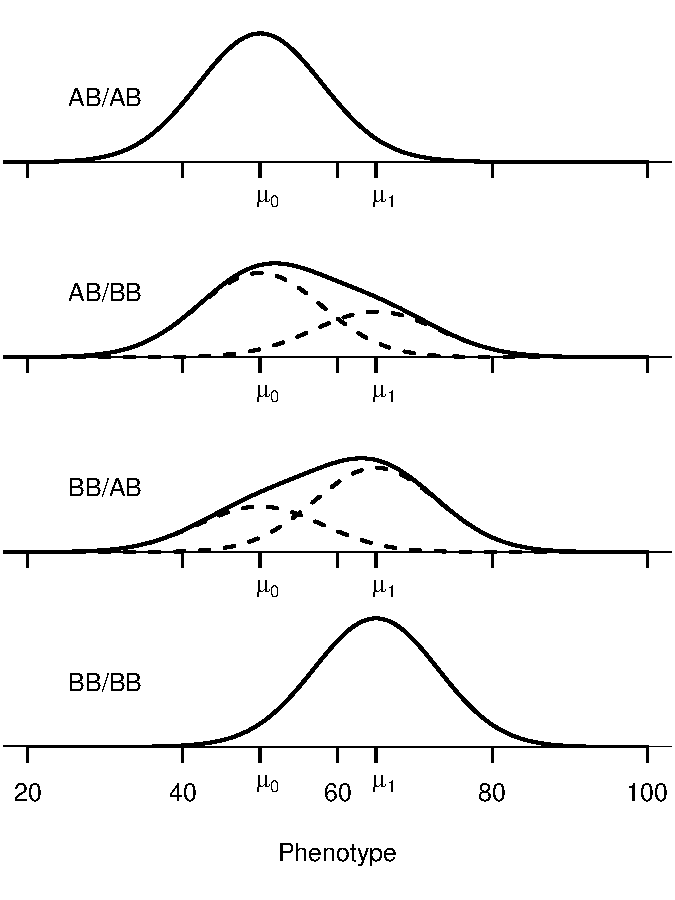
\includegraphics{Figs/mixtures_bw.pdf}
\end{minipage}




\newpage

\headsize \color{myyellow}
\hfill \begin{minipage}{5.75in}
\centering
Haley-Knott results
\end{minipage}

\vfill

\centerline{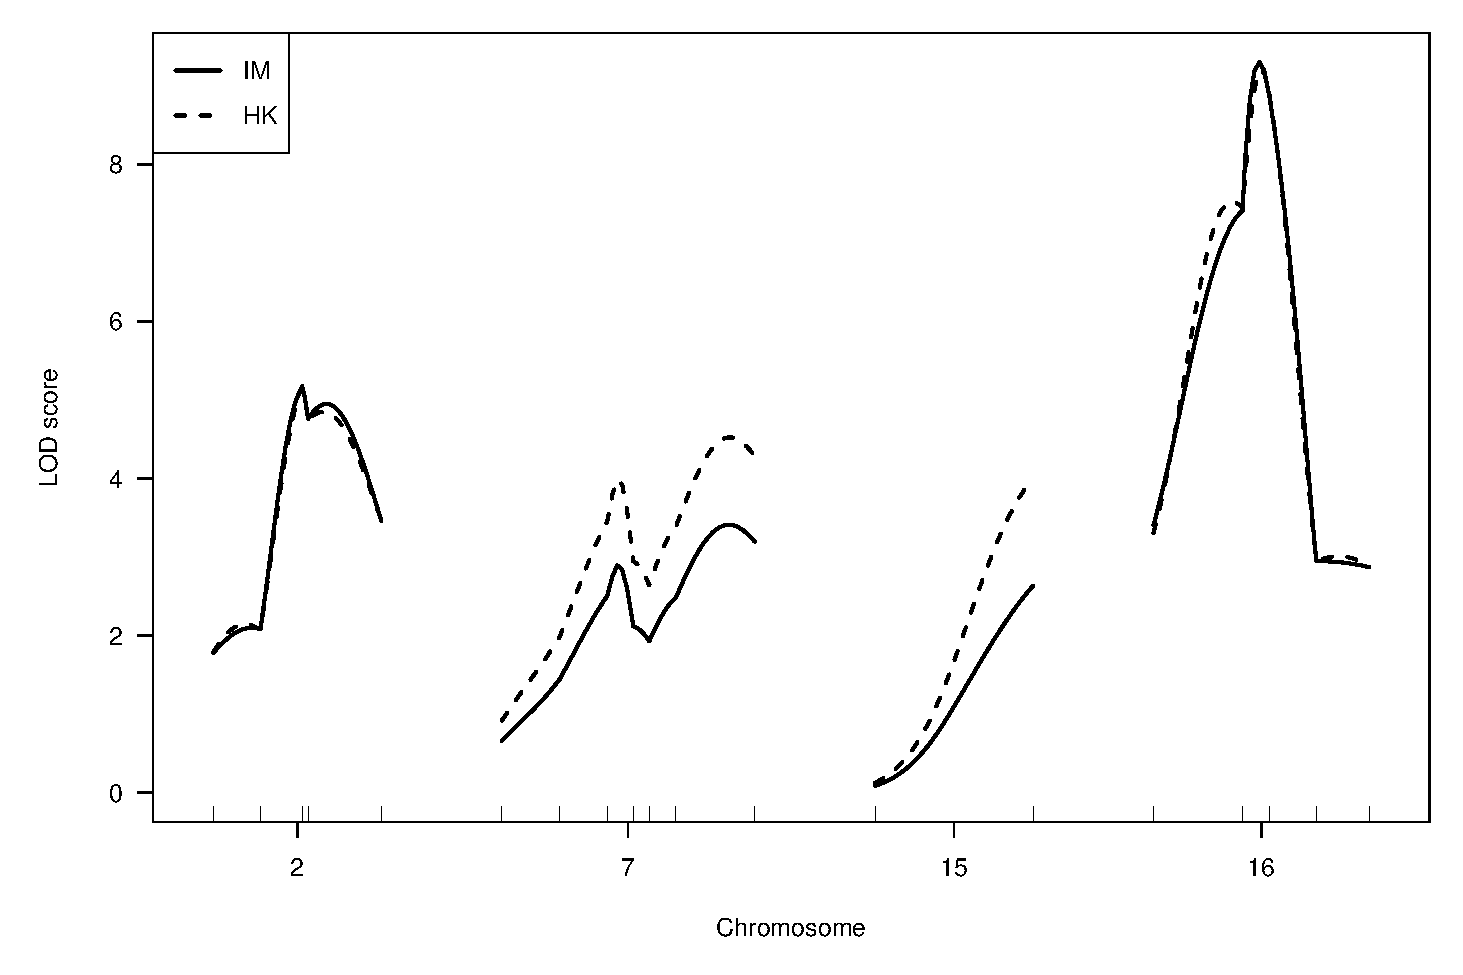
\includegraphics{Figs/hk_lod_bw.pdf}}



\newpage

\headsize \color{myyellow}
\hfill \begin{minipage}{5.75in}
\centering
H-K with selective genotyping
\end{minipage}

\vfill

\centerline{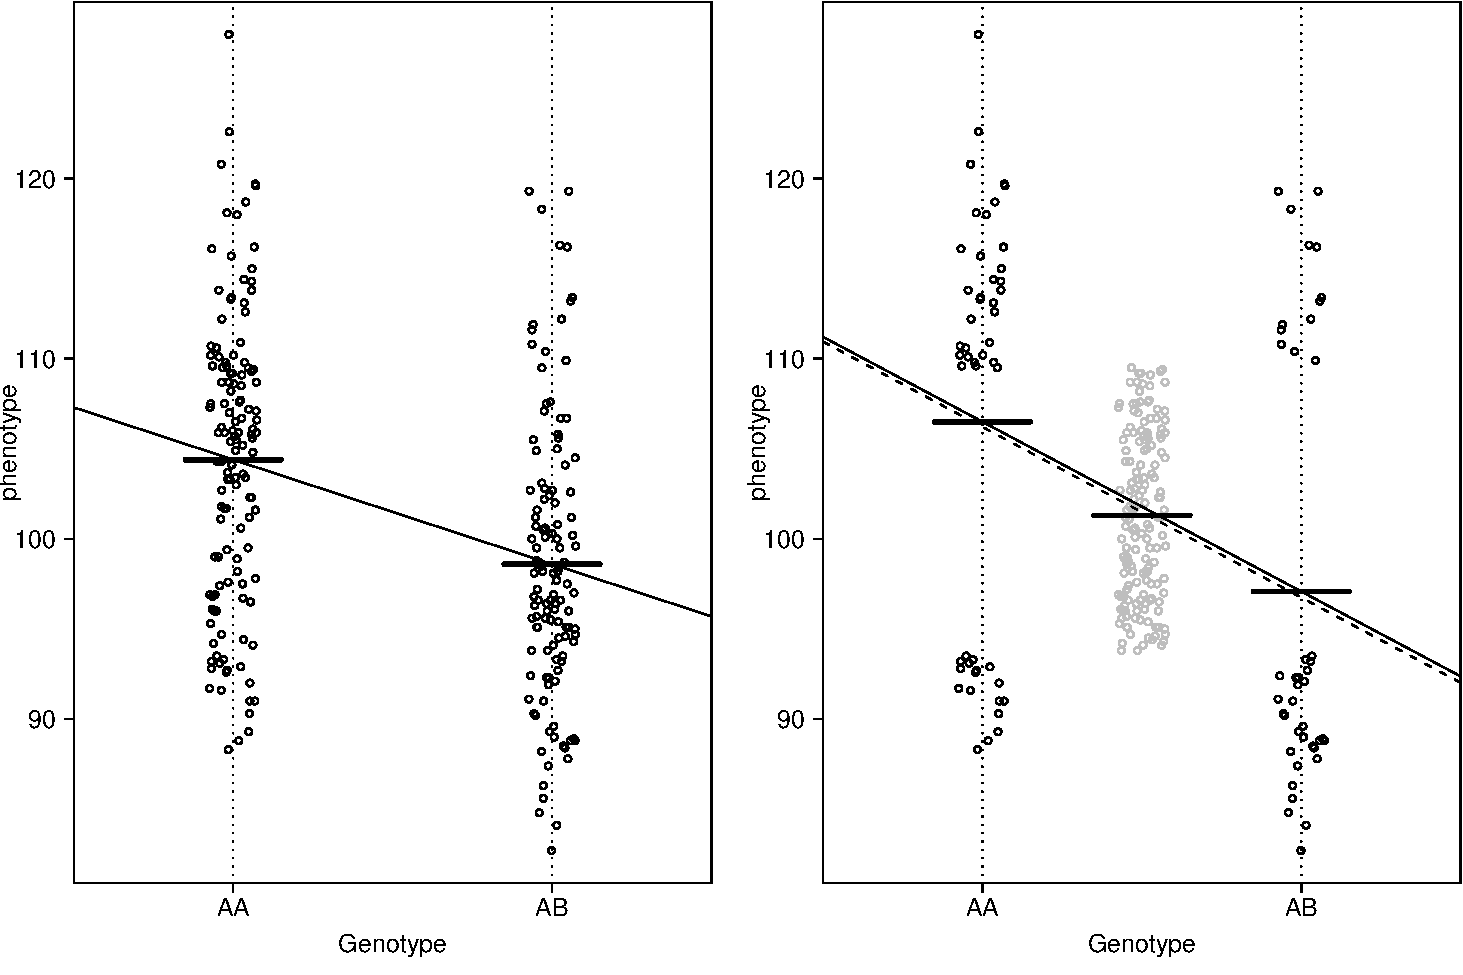
\includegraphics{Figs/hk_selgeno_bw.pdf}}




\end{document}
